\chapter{Discussion}\label{sec:7}

The present chapter summarises and discusses the results obtained in the preceding chapters.

\section{Input}\label{sec:08:1}

This chapter aimed to scrutinise the controlled VILLA input in order to appropriately contextualise the learner task in the linguistic tests discussed later on in the book.

The analysis of the association between case endings and the corresponding syntactic functions showed that, indeed, the ending -[a] is more strongly linked to the SUBJ function than the ending -[e] is linked to the OBJ function. This might play a role in justifying why learners hardly ever process the nominative case incorrectly, while errors concerning the accusative case are quite common. 

Further, while the object function was characterised by relatively high type variety, with numerous inanimate nouns performing it, the subject function is instantiated by only four macro-types, namely the two personal pronouns \textit{on} and \textit{ona}, ‘he’ and ‘she’, and masculine and feminine person names. The high type variety of the object function might explain why some learners managed to correctly inflect in the accusative case even nouns which never appeared in that form in the input. However, since the VILLA project was not designed to investigate this particular research question, it is impossible to pursue it any further based on the present data. 

The input was then scanned for all possible sentence models, described in terms of the combination of the following parameters:

\begin{itemize}
    \item word order: SO vs. OS;
    \item subject word class: personal pronoun, person name, common noun;
    \item object word class: person name, common noun;
    \item subject and object gender: masculine vs. feminine;
    \item animacy (animate vs. inanimate).
\end{itemize}

Not surprisingly, only a fraction of the 96 theoretically possible patterns were attested in the input. The trends highlighted by the analysis of type frequency were confirmed: the subject tends to be instantiated by personal pronouns or person names, while the object shows a privileged association with inanimate nouns. The target structures of the two structured tests are rare or absent altogether from the input when all parameters are considered: however, figures markedly rise when a morphological perspective is adopted, whereby word class and animacy are ignored (when legitimate) and patterns are considered as mere sequences of inflectional endings occurring in a given order.

The following sections aim to add a few details which may not emerge sufficiently from an exclusively quantitative analysis, such as the effect of information structure on the frequency of selected morphosyntactic structures. It further discusses the implications of the input distribution just reviewed for the learner task.

\subsection{Information structure}\label{sec:08:1.1}

The VILLA input was designed to allow for rigorous experimental control over a large set of variables, but at the same time it was delivered in the form of a communicative, interactive language course. In order not to sound unnatural, the teacher would inevitably produce the structures which she judged pragmatically most appropriate, even if these were \textit{not} the structures targeted in the language tasks. To exemplify, in a context in which the same known characters are mentioned over and over again, it is pragmatically appropriate to refer to them using personal pronouns or their names, like \textit{ona} ‘she’ or \textit{Julia}, rather than a common noun indicating their nationality of profession, like \textit{kucharka} ‘cook’. Together with the structure and contents of the course, this pragmatic constraint led to a very low frequency of constructions targeted in the VILLA structured tests, which exclusively include common nouns.

Across all models of transitive structures, pronouns and person names represent the lion's share as far as the expression of the subject function is concerned, while objects are mainly instantiated by inanimate nouns. This trend is not surprising if one considers the topics covered throughout the course, which for the most part described a handful of human characters along with their likes and dislikes and their relation with each other. Human referents clearly have the greatest chances of being the subject of transitive sentences for obvious extralinguistic reasons. The distribution of pronouns and person names to refer to the same human referent, in contrast, is regulated by information structure. In a typical VILLA input sequence \REF{ex:08:1}, pronouns are commonly used to refer to entities which have been previously introduced using a person name, although such topic maintenance is also frequently achieved by repeating the character’s name as well.

\ea%1
    \label{ex:08:1}
    \ea
    \label{ex:08:1a}
    \gll    \textit{{Juli-a} {lubi} {żółwi-a.}}\\
            Julia-\textsc{nom}  likes  turtle-\textsc{acc}\\
    \glt    ‘Julia likes the turtle.’
    \ex
    \label{ex:08:1b}
    \gll    \textit{{ona}   {lubi}   {lizaki}     {lubi}   {lizaki.}}\\
            She  likes  lollipops\textsc{.acc}   likes  lollipops\textsc{.acc}\\
    \glt    ‘She likes lollipops.’
    \ex
    \label{ex:08:1c}
    \gll    \textit{{ona}   {lubi}   {żółwi-a}   {i}   {lubi}   {czekolad-ę.}}\\
            She  likes  turtle-\textsc{acc}  and  likes  chocolate-\textsc{acc}\\
    \glt    ‘She likes turtle and chocolate.’
    \z
\z

Entities are mainly introduced using person names rather than common nouns for reasons related to discourse. This claim can be best instantiated on the grounds of the context in which the class is working on the PowerPoint slide in \figref{fig:08:1}, trying to decide what course character likes or owns each of the objects depicted therein. 

\begin{figure}
    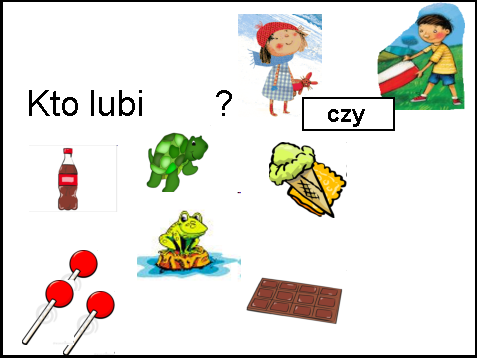
\includegraphics[width=\textwidth]{figures/08-1.pdf}
    \caption{PowerPoint slide from the VILLA input}
    \label{fig:08:1}
\end{figure}

Based on information previously provided during the lesson, the learners can decide between Julia and Filip (top right), both well known course characters. In this particular communicative context the objects represent the discourse topic, while the two children are in the focus position. The sequence opens with the utterances in \REF{ex:08:2}:

\ea%2
    \label{ex:08:2}
    \ea{\label{ex:08:2a}
    \gll    \textit{{kto}   {lubi}   {czekolad-ę}}?\\
            who   likes   chocolate-\textsc{acc}?\\
    \glt    ‘Who likes chocolate?’
    \ex\
    label{ex:08:2b}
   \textit{ {eh}   {Gaston}}\footnote{Gaston is the pseudonym of one of the learners.}?
    \ex
    \label{ex:08:2c}
    \gll    \textit{{tak}   {Juli-a}     {lubi}   {czekolad-ę.}}\\
            Yes  Julia-\textsc{nom}  likes  chocolate-\textsc{acc}\\
    \glt   ‘Yes, Julia likes chocolate.’
    \ex
    \label{ex:08:2d}
    \gll    \textit{{czekolad-ę}     {lubi}   {Juli-a.}}\\
            chocolate-\textsc{acc}  likes  Julia-\textsc{nom}\\}
    \glt    ‘Julia likes chocolate.’
    \z
\z

The teacher first asks Gaston who likes chocolate, whether Julia or Filip. Input transcription at this stage is only available for the teacher's speech and does not comprise the learner's response, but only teacher feedback. Judging on the teacher's third turn, however, Gaston's answer must have been correct, at least in terms of content; in any case, the teacher repeats (or recasts) the learner’s response. Even though the topic \textit{czekoladę} ‘chocolate-\textsc{acc’} performs the object function, thus licensing syntactically marked word order, the native speaker at first prefers to produce a syntactically unmarked SO sentence, in which pragmatic markedness is expressed prosodically through the stressing of utterance-initial \textit{Julia}, which highlights her as the sentence focus. Only later will the teacher produce the equivalent OS utterance.

Judging on the apparent interchangeability of the two word orders, one may wonder if learners even deemed it necessary to pay attention to such syntactic devices, since different syntactic structures correspond to identical meaning. Speakers of languages which also allow the functional manipulation of word order, like German and, with different means, Italian, might even have found this apparently random use of syntactically marked structures a little odd. On the other hand, the school-like context in which the project was carried out might have prompted students to pay attention to these details of the target grammar even if it seemed difficult to associate competing forms to the corresponding meaning.

This example is precious to understand two important points. First, not only are OS sentences more marked than their SO equivalents, but their purpose can be easily (and perhaps, preferably) fulfilled by other strategies to mark departures from the default alignment between the syntactic and pragmatic structure of the utterance (topic-subject; focus-object).

On the other hand, the example clarifies why person names are so much more frequent than common nouns in transitive structures. Teacher speech is mainly based on PowerPoint slides which depict the same characters over and over again. Thus, even if each course character is identified by a particular nationality and profession, expressed in turn by common nouns, the course characters become so familiar that it would seem somewhat unnatural to refer to them otherwise than by their name, for instance by saying \textit{dziewczynka} ‘little girl’ instead of just \textit{Julia}. In contrast, the target sentences of the EI task required learners to process common nouns in the absence of any context, something which they could arguably be ill-equipped to do at such an early stage of acquisition and on the sole basis of the input just described.

\subsection{Form–function association}\label{sec:08:1.2}

The analysis of form–function associations has shown that, based on a statistical analysis of the input, it is simpler to associate -[a] to the subject function than -[e] to the object functions. Before moving on to a more detailed discussion of the mechanisms of such an analysis, it seems worthwhile to point out a few important details which may prove helpful to provide a more comprehensive picture of the learner’s task in the VILLA project.

The first is that while subconscious input analysis and associative learning certainly play a role in SLA, there are many other factors which may concur to explain learner behaviour. As far as the nominative case in -[a] is concerned, for instance, it most often coincides with the citation form of lexical items, i.e. the form which was usually introduced first throughout the course and which was used out of context. To exemplify, \textit{kuchnia} ‘cuisine’ is a noun which due to its semantics tends to occur in the accusative case, yet, its basic word form is modelled on the nominative case: in example \REF{ex:08:3}, the teacher first uses the noun in the accusative case, then asks the class to repeat it aloud in the nominative.

\ea%3
    \label{ex:08:3}
    \ea
    \label{ex:08:3a}
    \gll    \textit{{ona}   {lubi}   {kuchni-ę}   {włosk-ą.}}\\
            she  likes  cuisine-\textsc{acc}  Italian-\textsc{acc}\\
    \glt    ‘She likes Italian cuisine.’
    \ex
    \label{ex:08:3b}
    \gll    \textit{{proszę}   {mówić}   {kuchni-a}   {włosk-a.}}\\
            please  say  cuisine-\textsc{nom}  Italian-\textsc{nom}\\
    \glt    ‘Please say Italian cuisine.’
    \z
\z

Similar factors, while not quantitative in nature (a word initially introduced in the nominative case may be then used predominantly in the accusative case, e.g. \textit{herbata} ‘tea’) certainly contribute to the prominence (here understood as the possibility of remembering it) of one or another form. 

Further, widespread morphological syncretism may hinder the univocal identification of form–function associations. In perfectly legitimate sentences like \REF{ex:08:4a} and  \REF{ex:08:4b}, nouns performing different syntactic functions are marked by the same inflectional ending -[a] because they belong to different inflectional paradigms. Curiously, in this respect such utterances resemble those produced in the EI test by learners who cannot yet manipulate inflectional morphology (\ref{ex:08:4c}, here transcribed in standard orthography).

\ea%4
    \label{ex:08:4}
    \ea\label{ex:08:4a}
    \gll    \textit{{siostr-a}   {woła}   {brat-a}} \\
            sister-\textsc{nom} calls   brother-\textsc{acc}\\
    \glt    ‘The sister calls (her) brother.’
    \ex\label{ex:08:4b}
    \gll    \textit{{ona}   {ma}   {brat-a.}}\\
            she  has  brother-\textsc{acc}\\
    \glt    ‘She has a brother.’
    \ex[*]{\label{ex:08:4c}
    \gll    \textit{{dziewczynk-a}   {ciągnie} {portugalk-a}}\\
            little.girl-\textsc{nom}  pulls   Portuguese.woman-\textsc{nom}\\}
    \glt   
    \z
\z

The two models can only be distinguished based on the grammatical gender and animacy of the two nouns involved, because the endings they exhibit are formally identical. This may easily confuse learners, as it adds a further factor to take into consideration when computing the form–function association between case endings and syntactic functions: not only is the syntactic function relevant, but grammatical gender also needs to be accounted for. This in turn is not predictable, although in the case of human nouns it almost always coincides with biological sex. There are exceptions to this rule, though: in \REF{ex:08:5}, both the subject and the object are realised by nouns inflected according to the feminine paradigm, namely \textit{córka}, ‘daughter’ and \textit{tata}, ‘Dad’. The latter, however, is semantically masculine. Nevertheless, it should be pointed out that although fairly frequent, the word \textit{tata} is the only lexical item characterised by such properties.

\ea%5
    \label{ex:08:5}
    \gll    \textit{{córk-a}     {Juli-a}     {kocha} {tat-ę.}}\\
            daughter-\textsc{nom}  Julia-\textsc{nom}  loves  dad-\textsc{acc}\\
    \glt    ‘(The) daughter Julia loves (her) father.’
    \z

A further point of complexity in the VILLA input is represented by the fact that in Polish the default case of direct objects under the scope of negation is not the accusative, as one would expect, but the genitive. In the paradigm of masculine animate nouns, the -[a] ending characterises both the accusative case and the genitive \REF{ex:08:6a}. In the feminine paradigm, on the contrary, the two endings are clearly distinct, so that direct objects are marked by different case endings depending on whether or not their verb is negated \REF{ex:08:6b}. Finally, the genitive is also the case in which the subject appears when an existential verb is negated \REF{ex:08:6c}.

\ea%6
    \label{ex:08:6}
    \ea\label{ex:08:6a}
    \gll   \textit{ {nie}   {ona}   {nie}   {kocha}   {dziadk-a}   {Karol-a.}} \\
            no  she  not  loves  grandpa-\textsc{gen}  Karol-\textsc{gen} \\
    \glt    ‘No, she doesn't love grandpa Karol.’
    \ex\label{ex:08:6b}
    \gll    \textit{{babcia}   {nie}   {lubi}   {muzyk-i.}}\\
            grandmother  not  likes  music-\textsc{gen}\\
    \glt    ‘Grandmother doesn't like music.’
    \ex\label{ex:08:6c}
    \gll    \textit{{nie}  {ma}  {Karol-a}}\\
            not  has  Karol-\textsc{gen}\\
    \glt    ‘Karol is not here.’
    \z
\z

The last example is crucial in that it confuses the relation between syntactic function and inflectional ending. These regularities are quite systematic and easily described if basic meta-linguistic concepts and rules are introduced, but the VILLA input included no such explanations. 

Another important point concerns the selection of the meaning engaged in the form–function association. In the present analysis “subject” and “object” were chosen because they correspond most accurately to the meaning expressed in Polish by the morphemes -[a] and -[e], respectively. There is no guarantee that the learner identified the same relation, however: in fact, it may be argued that such top-down expectations resemble \citegen{Bley-Vroman1983} comparative fallacy, whereby the interlanguage is analysed not in terms of its internal organisation, but of the target it is supposed to imitate. In fact, different learners may assign different meaning to the same morpheme. \citet{Bernini2018a} and \citet[28-33]{Dimroth2018} both discuss two forms of the word \textit{strażak} ‘fireman’ as can be encountered in narrations produced within the Italian and German VILLA editions, respectively, whereby a form in \textit{{}-k} (e.g. [ˈstraʒak]) modelled on the nominative case opposes a form in \textit{{}-em} (e.g. [straˈʒakjem]), modelled on the instrumental case \textit{strażakiem}. In the Italian data, the opposition seems to vehiculate the functions “subject/controller” vs. “oblique”, while in the German data a “singular” vs. “plural” seems more probable.

The learner’s task is further complicated by the differential object marking (DOM) encountered in the masculine paradigm. Nouns referring to things appear in a form identical to the nominative case, characterised by a zero morph attached to the consonantal stem (\ref{ex:08:7a} and \ref{ex:08:7c}), while the accusative case of masculine animate nouns \REF{ex:08:7b} present an -[a] ending \REF{ex:08:7d}, which is also found in the genitive case \REF{ex:08:7e}. This last observation highlights the fact that DOM complicates the association between form and function on metalinguistic, rather than statistical grounds: on hearing the two forms in \REF{ex:08:7d} and \REF{ex:08:7e}, the learner can be hardly expected to identify a comprehensive morphosyntactic rule, especially in the absence of an understanding of the category of case and detailed information as to Polish inflectional morphology. It must be said, however, that all VILLA L1s except German do not inflect nouns for case, so that encountering the same word form in different syntactic functions should not be particularly problematic for speakers of these languages. Nonetheless, the typological difference between the VILLA L1s and Polish is quite evident and a provisional hypothesis should be formulated to account for it. 

\ea%7
    \label{ex:08:7}
    \ea\label{ex:08:7a}
    \gll    \textit{{to}    {jest}  {balonik{}-${\emptyset}$}}\\
            this\textsc{.nom}  is  balloon\textsc{-nom}\\
    \glt    ‘This is a balloon.’
    \ex\label{ex:08:7b}
    \gll    \textit{{to}    {jest}  {strażak-${\emptyset}$}}\\
            this\textsc{.nom}  is  fireman\textsc{-nom}\\
    \glt    ‘This is a fireman.’
    \ex\label{ex:08:7c}
    \gll   \textit{ {Jan-${\emptyset}$    ma  balonik-${\emptyset}$}}\\
            Jan\textsc{-nom}  has  balloon\textsc{-acc}\\
    \glt    ‘Jan has a balloon.’
    \ex\label{ex:08:7d}
    \gll    \textit{{Jan-${\emptyset}$    zna  strażak-a}}\\
            Jan\textsc{-nom}  knows  fireman\textsc{-acc}\\
    \glt    ‘Jan knows a fireman.’
    \ex\label{ex:08:7e}
    \gll    \textit{{to}    {jest}  {samochód-${\emptyset}$}  {strażaka}}\\
            this\textsc{.nom}  is  car\textsc{-nom}  fireman\textsc{-gen}\\
    \glt    ‘This is the fireman's car.’
    \z
\z

A final point concerns the form component. Discussing the form–function association between -[e] and "object”, it was stated above that i) most feminine nouns in the accusative case are characterised by word-final -[e], and ii) only a small proportion of words in -[e] are indeed instances of ACC.SG.F. While i) seems unproblematic, ii) may not seem entirely adequate to model the learner’s task during input processing. This point begs the researcher to take a stance, depending upon the answer to the following question: when establishing form–function associations through contingency learning, can learners distinguish words sharing a given form, but belonging to obviously different word classes, and treat them in a different manner? Since in the tasks discussed in this work the VILLA learners were required to process nouns referring to human beings, one of their goals was to identify the forms (i.e. the inflectional endings) in which such words may appear, possibly attempting to discern any regularity governing their distribution. Thus, in the case of ACC.SG.F -[e] one may wonder whether it is relevant to know how many input \textit{words} in -[e] really encode human nouns in the accusative case, or whether it is only relevant to know how many \textit{human nouns} in the input end in -[e]. 

In the former case, the learner will need to analyse all words in -[e] which comprise feminine nouns, indeed (e.g. \textit{portugalk-ę} ‘Polish.woman-\textsc{acc.sg’}), but also verbs (\textit{idzie} ‘go.\textsc{pres.3sg’}) adverbs (\textit{dobrze} ‘well’), adjectives (\textit{jakie} ‘which.\textsc{nom/acc.sg.n}’) and conjunctions (\textit{ale} ‘but’). Upon encountering a word in —[e], learners will (subconsciously) note whether or not it encodes the target meaning, in answer to the implicit question “how often do words in -[e] represent feminine human nouns in the object function?”.

In an alternative scenario, learners will separate nouns from all other categories and simply compute a list of the possible endings of human nouns along with their relative frequency (how many nouns with human referents are characterised by word-final -[e]? How many by —[a]? and so on).

The consequences of this decision for the estimation of form–function association are important. 

If learners are assumed to be able to distinguish word classes, then only a subset of input words sharing the form under investigation should be considered in the computation of form frequency, which will result in a higher form–function association index, all other things being equal. To exemplify, the range of words in -[e] relevant for the meaning “accusative case of feminine nouns” would comprise e.g. \textit{portugalk-ę} ‘Polish.woman-\textsc{acc.sg’}, but not \textit{idzie} ‘go.\textsc{pres.3sg}’, \textit{dobrze} ‘well’, \textit{jakie} ‘which.\textsc{nom/acc.sg.n}’ or \textit{ale} ‘but’, despite the fact that all share the form of interest -[e]. If learners cannot distinguish word classes, in contrast, then the same count should comprise any word in -[e].

In order to accurately acknowledge the fact that input processing may be selective, it seems appropriate to compute function > form associations based on language exemplars in which the meaning in question is present. From this perspective, the learner’s task is to identify how many feminine nouns in the object function  are characterised by word-final -[e], and how many are not. 

When this rationale is applied to the VILLA data, the surprising results presented in \tabref{tab:08:1} and \tabref{tab:08:2} are obtained. Note that these tables are an elaboration of \tabref{tab:03:1} and \tabref{tab:03:2}, respectively, in which the columns no longer relevant have been shaded: in fact, following the approach adopted in this section, form–function association is simply the ration between the number of words including both form and function and the number of words encoding function regardless of form. Both association indexes are close to 1, which indeed reflects the fact that in the peculiar VILLA input most NOM.SG.F are characterised by word-final -[a], and most ACC.SG.F are characterised by word-final -[e].

\begin{table}
    \begin{tabularx}{\textwidth}{X>{\columncolor{lsDOIGray}}rrr >{\columncolor{lsDOIGray}}rr>{\columncolor{lsDOIGray}}r}
        \lsptoprule
        a & b & c & d & e & f & g\\
        \midrule
        L1 & {}-[e] & \textsc{Acc} \textsc{fem} & \textsc{Acc} \textsc{fem} -[e] & d/b & d/c & e*f\\
        EN & 6541 & 441 & 415 & 6.34\% & 94.10\% & 5.97\%\\
        FR & 3789 & 365 & 345 & 9.11\% & 94.52\% & 8.61\%\\
        GE & 6424 & 414 & 379 & 5.90\% & 91.55\% & 5.40\%\\
        IT & 7675 & 624 & 598 & 7.79\% & 95.83\% & 7.47\%\\
        NL & 6570 & 519 & 494 & 7.52\% & 95.18\% & 7.16\%\\
        \lspbottomrule
    \end{tabularx}
    \caption{Form > function index for syntactically relevant contexts only, ACC.SG.F -[e]}
    \label{tab:08:1}
\end{table}

\begin{table}
    \begin{tabularx}{\textwidth}{Xrrr rrr}
        \lsptoprule
        a & b & c & d & e & f & g\\
        \midrule
        L1 & {}-[a] & \textsc{Nom} \textsc{fem} & \textsc{Nom} \textsc{fem} -[a] & d/b & d/c & e*f\\
        EN & 7091 & 2471 & 2437 & 34.37\% & 98.62\% & 33.89\%\\
        FR & 4239 & 1798 & 1730 & 40.81\% & 96.22\% & 39.27\%\\
        GE & 7100 & 2338 & 2265 & 31.90\% & 96.88\% & 30.91\%\\
        IT & 9345 & 3198 & 3161 & 33.83\% & 98.84\% & 33.43\%\\
        NL & 7483 & 2787 & 2721 & 36.36\% & 97.63\% & 35.50\%\\
        \lspbottomrule
    \end{tabularx}
    \caption{Form > function index for syntactically relevant contexts only, NOM.SG.F -[a]}
    \label{tab:08:2}
\end{table}

This observation however is in stark contrast with the results of the tasks discussed in this work, which clearly show that -[a] tends to be overextended onto -[e] by a vast number of learners. It seems, therefore, that form–function association may not be the most influential factor to determine which input word-form will be selected as the basic word-form of the learner variety. Based on the tables presented above, raw token frequency appears to be a good candidate, as the instances of -[a] NOM are almost six times as frequent as -[e] ACC. Moreover, the nominative case appears in a much larger number of contexts than the accusative case, and is the default citation form of nouns. In sum, the approach adopted here in order to model learner selectivity in the computation of form–function association appears heavily biased by the fact that raw frequency is not taken into account. 

\subsection{A learner variety perspective}\label{sec:08:1.3}

As \citet{Dimroth2018} points out, it is often difficult to draw a line between the claims and predictions of the learner variety approach and usage-based theories. As far as the input is concerned, particularly, both consider it an essential component for interlanguage development, the raw material which the learner communication faculty will shape in order to reach the set communicative objectives.

From this perspective, inflectional morphology seems by no means indispensable to interpret input sentences, although it certainly is a characteristic and obligatory feature of the target language. It is not surprising then that learners can easily do without it and still communicate effectively, especially when a context is available. The analysis of learner’s semi-spontaneous productions has clearly shown that semantics (animacy) and default SO (controller — theme) word order are usually sufficient to express the simple meaning required in the VILLA tasks. 

The same trends are also commonly encountered in a vast proportion of input utterances: SO structures are preferred even in a language such as Polish, with its complex nominal morphology and the theoretical possibility to manipulate word order at will. By the same token, agents tend to be animate and patients tend to be inanimate simply because situations usually present this structure. In other words, the principles of utterance organisation in question may be seen as a feature of the basic variety, but are commonly encountered in most instances of verbal communication.

The models corresponding to the target sentences of the structured tests were either absent or rare in the input, precisely because they purposefully eliminate all natural cues to sentence organisation with the exception of inflectional morphology. From a communicative point of view, then, the EIT and the comprehension tasks are little more than exercises targeting meta-linguistic skills. The communicative principles of the basic variety are hardly applicable, but on the other hand it can be argued that there is hardly any meaning to express. 

Since the VILLA participants are all adult, competent speakers of at least one L1, one could argue that their experience in terms of pragmatics and world knowledge may sometimes prevail on the input received. As shown in a study conducted on copular structures \citep{Saturno2015}, learners often choose to ignore highly frequent input patterns, developing their own interlanguage structures instead. The copular construction with \textit{to} ‘this’, though extremely common in the input, appeared to be disfavoured both in a structured test and in semi-spontaneous production \citep{Saturno2018}. In the latter context, learners creatively elaborated new, ungrammatical constructions. The structure in \REF{ex:08:8a} probably has its models in \REF{ex:08:8b} and \REF{ex:08:8c}.

\ea%8
    \label{ex:08:8}
    \ea{\label{ex:08:8a}
    \gll    [ɔna   jɛst   dʒovanna].\\
            She  is  Giovanna\\}\jambox*{(5112)}
    \glt    ‘She is Giovanna.’
    \ex\label{ex:08:8b}
    \gll    {to}    {jest}  {Anna}\\
            this\textsc{.nom}  is  Anna\textsc{.nom}\\
     \glt    ‘This is Anna.’
    \ex\label{ex:08:8c}
    \gll    {Anna}  {jest}  {polką}\\
            Anna  is  Polish.woman\textsc{.ins}\\
     \glt    ‘Anna is a Polish woman.’
    \z
\z

In sum, from the perspective of the learner variety approach the results of the linguistic tasks are not particularly unexpected. In the language tasks inflectional morphology is hardly encountered because it is not part of the repertoire of early interlanguages, which prefer to rely on semantics and word order. The same preferences contribute to shaping the input, too, although the latter obviously includes all obligatory traits of the target language, such as inflectional morphology. 

\section{The elicited imitation task}\label{sec:08:2}

Perhaps the most self-evident result emerging from the analysis of the Elicited Imitation Task (EIT) is that, as expected based on input analysis, the NOM ending -[a] shows a marked tendency to overextend onto ACC -[e]. For most participants, -[a] is indeed the only ending produced, and thus the basic form of nouns, which — if one accepts the theoretical premises of the EI test — should clearly point to a positional principle of utterance organisation, whereby syntactic functions are determined by the relative position of nouns in the utterance.

A much smaller number of learners produce target-like output, in which the endings -[a] and -[e] alternate depending on the syntactic function of the noun. Such performance — again, based on the theoretical premises of the task — should indicate that the target language morphosyntactic principle of utterance organisation has been correctly identified and can be successfully reproduced in the output. Finally, a set of participants exhibits a variety of complex scenarios. 

Word order was found to exert a powerful role, whereby OS targets appear to cause greater difficulties than their SO equivalents. Time of exposure was also shown to be an important factor, whose predictable effect is an increase in performance from T1 from T2, with numerous learners moving closer to the target morphosyntactic principle of utterance organisation. An interaction with word order is observed, too: if partial improvement occurs, it is more likely to be on SO than OS targets. Finally, a weak but significant correlation was found between the LLama test and the score for the repetition of -/e/, averaged for time and word order.

Against this general picture, a few points remain partially unclear. They can be summarised as follows:

\begin{itemize}
    \item The range of observed case endings;
    \item Role of word order and processing for meaning;
    \item better performance on -[e] than -[a] targets;
    \item better performance at T1 than T2 targets.
\end{itemize}

It seems that all these issues ultimately depend on a precise understanding of the mechanism of the EIT, which is itself not completely clear. Therefore, the discussion will start with an attempt to identify the level of analysis into which the EI test may be thought to tap. 

\subsection{Range of case endings}\label{sec:08:2.1}

The range of case endings produced by the learners seems to be quite restricted. Such observation is not in accordance with studies on the morphological development in Slavic languages, which suggest that learners first go through a NOM/non-NOM opposition, and only later do they stabilise this generic contrast into a more target-like NOM/ACC distinction (see \chapref{sec:1}.

This does not necessarily mean that the VILLA learners acquired case marking better and more quickly than untutored SLA learners. The analysis of the VILLA semi-spontaneous production data by \citet{Bernini2016} and \citet{Dimroth2018} shows that utterance structure simultaneously reflects a variety of principles which in spontaneous SLA are typical of different developmental stages, such as the pre-basic variety’s pragmatic structure ``focus last''; the basic, semantic ``controller first''; and the post-basic SVO syntactic organisation. Interpreting such mixture of apparently anachronistic principles as a consequence of the particular VILLA learning context, one could propose the label ``Instructed Basic Variety''. Bernini in particular correlates the structural properties of the interlanguage with its phonology, arguing that while random phonological variability, or rather tolerance towards allophonic variation is typical of pre-basic varieties, ``la fixation d’une forme de base du […] mot dans la variété basique réduit la gamme de variation (allo-)phonique […], en fondant la possibilité d’oppositions phonémiques''. In this respect, he also observes that while several lexical items are relatively stable in their phonological form, others show considerable variability, both in their supposed target and in their phonetic structure, e.g. \{ɕpi, ʃpi, spi\} for target /ɕpi/, ‘sleeps’. Even when the various tokens produced by a learner seem to be mappable onto specific target forms, and thus to reflect the input to a certain extent, their use is nonetheless functionally differentiated, as it has been shown to be the case with spontaneous SLA (\citealt{BroederEtAl1993}). Moreover, Bernini suggests four factors which may have an influence in determining the phonological variability of lexical items in initial SLA, namely a) frequency, b) the number and structure of syllables, c) the number of different word-forms present in the input, and d) semantics. While b) and d) are intrinsic to the lexical items, a) and d) depend on the input. This wealth of data only makes it harder to interpret the output of the EI task, as even the correct repetition of case endings may indicate a post-basic syntactic utterance organisation just as well as pre-basic, random phonological variability. What appears to be incontrovertible is that learners must have picked these alternative endings from the appropriate input paradigms, thus showing some sensitivity to it. If one excludes the instances of centralised vowels mainly produced by the German learners, virtually all endings produced are instances of -[a] or -[e], despite the fact that the relevant paradigm also includes other salient and frequent endings, such as INS [o\~{w}]. This observation would witness to the fact that learners identified the syntactic context in which the endings -[a] and -[e] may occur, namely transitive sentences, and conversely that they are aware that in that syntactic context only those endings are allowed.

On the other hand, the fact that only -[a] and -[e] occur in the EI data is hardly surprising if one accepts that there might be repetition without processing, whereby learners only repeat what they hear without accessing their L2 grammar. In this situation, only two endings occur in the output simply because only those endings are present in the stimulus sentences.

\subsection{Sources of error: processing for meaning vs. perception}\label{sec:08:2.2}

Compared to previous studies using the EIT, the target structure of the present work introduces additional variables which increase the complexity of the analysis and interpretation of the data. Case marking poses different challenges from other target structures which only affect grammatical correctness, like for instance verb placement as studied by \citet{Håkansson1989} or \citet{Schimke2011}. Unlike case marking, the position of a verb in the utterance is not likely to change the overall meaning of the sentence. 

In addition, the data produced by the VILLA EIT are limited to the learner’s final output. In the absence of a comprehension or translation test, it is impossible to tell what learners meant to say. This is unfortunate, as the output of the EIT is the product of at least three complex processes, namely perception, comprehension and production: errors may lie at any level. By observing the learners’ processing of an OS target, for instance, one cannot tell if the underlying grammatical meaning was identified, firstly, and if any effort was made to reproduce it, secondly. It is also impossible to rigorously exclude that learners performed the task without processing targets for meaning. Indeed, this suspicion is further reinforced by the weak but significant correlation between phonological memory capacity as measure by the LLama test and the scores in the repetition of -/e/.

These questions were dealt with in detail in \chapref{sec:6}, in which the results of the EI and of the comprehension test were correlated in an attempt to provide a comprehensive picture of learners’ processing skills, and will be discussed further in \sectref{sec:08:4}. For the time being, this section will focus on the clear effect of word order as observed in the EIT alone.

The rationale of word order manipulation in the EIT was that SO targets, being syntactically and pragmatically unmarked, should be easier to process than their marked OS counterpart. This claim is founded on a variety of reasons discussed in \chapref{sec:1}, ranging from the typological diffusion of SO as opposed to OS word order, to acquisitional data showing that case marking first develops in SO sentences, to the input analysis presented in \chapref{sec:3}, which shows that even within the strictly experimental conditions of the VILLA project, the vast majority of transitive utterances are characterised by an SO structure.

However, understanding the direct impact of these general constraints on the EIT implies a few argumentative steps. For learners to find OS targets harder than their SO equivalent, it is necessary that they can recognise them as such, which is not obvious. When the OBJ is repeated incorrectly, it receives a basic ending in -[a], just like the noun performing the SUBJ function. As both nouns are now marked by an identical ending, what matters to express meaning is their relative position, the first being the SUBJ, the second the OBJ. To express the meaning of the OS target using a positional principle, the learner would need to swap the two nouns: yet this only happens once across the whole corpus. Two alternative accounts may be proposed. The first is that learners understand the OS structure of the target, but since they cannot express the desired meaning using inflectional morphology, they simply renounce to express it at all. This produces an utterance which indeed seems to express a completely different meaning based on a positional principle. The other explanation is that learners producing non-target-like case-marking could \textit{not} identify the OS structure of the target, and either interpreted it as an SO structure, or simply recognised the lexical items involved without any further specification of their grammatical role, by using an invariable word form ending in -[a]. 

In both cases, it seems that the learners renounced to express the specific meaning of the target sentence, agreeing to repeat a sentence which either did not correspond to the meaning they had identified, or did not corresponded to any meaning at all. Surely this is a powerful argument against the hypothesis that the EIT can be used to approximate spontaneous speech while retaining full control over the target structure. Although not a single learner commented on not being able to express what was really meant, it must be said that because of their lack of context and abstractness, the target structures of the EIT may seem to express a very abstract, generic meaning anyway. 

Even if one accepts that learner output may not express any meaning, at least not syntactic, it still remains to be explained why repetition scores are consistently lower on OS than SO targets, although in a situation in which test-takers do not associate case endings to the corresponding syntactic functions, it does not even seem legitimate to speak of word order. Since -[a] and -[e] do not correspond to SUBJ and OBJ, but are merely two segments, why should there be a difference in scores depending on which one comes first in the stimulus sentence?

The answer may come from perceptual prominence, which in turn is closely related to saliency, however understood: the present work adopts \citegen[1030]{Peters1985} argument that only salient stretches of sound constitute reasonable candidates for extraction from the input string, extraction in turn being defined as the recognising and remembering of language elements. This view is projected against the wider picture of child language acquisition by \citet[1164]{Slobin1985}: 

\begin{quote}
on the most basic level, accessibility of linguistic material can be defined in terms of ‘perceptibility’. That is to say, the only linguistic material that can figure in language making are stretches of speech that attract the child’s ‘attention’ to a sufficient degree to be noticed and held in memory.
\end{quote}

Data on earlier EI task studies show that, indeed, perception may be a relevant factor in explaining the results of this task. \citet{GallimoreTharp1981} state that the accessibility of linguistic elements depends on their position in the utterance according to the hierarchy initial > final > medial. \citet{Peters1985} and \citet[1166]{Slobin1985} suggest that utterance-initial and utterance-final positions are maximally prominent and accessible for segmentation and storage, whereas utterance-internal positions are harder to access. \citet[300]{VanPatten2000} proposed his operating principles P4 (learners first process elements in sentence/utterance initial position) and P4a (learners process elements in final position before elements in medial position). Finally, and most relevantly for the present work, \citet[151]{Rast2008} found that the accuracy of word repetitions in initial L2 Polish is affected by word position (utterance initial and final vs. medial) independently of the time of exposure (0, 4 and 8 hrs). 

These studies typically considered the perceptual prominence of entire words or free morphemes. But the same rationale can be applied to inflectional morphemes, which for a learner who does not process targets for meaning are indeed mere segments. In terms of perceptual prominence, in SO sentences the ACC ending -[e] occurs in utterance-final position, thus gaining maximal prominence \REF{ex:08:9a}. In OS sentences, in contrast, this element always occurs in utterance-medial position, which might make it harder to perceive and consequently reproduce \REF{ex:08:9b}.

\ea%9
    \label{ex:08:9}
    \ea\label{ex:08:9a}
    \gll    [nauʧɨʨelk-a   pxa    studentk-e].\\
            teacher-\textsc{nom}  pushes  student-\textsc{acc}\\
     \glt    ‘The teacher pushes the (female) student.’
    \ex\label{ex:08:9b}
    \gll    [studentk-e   pxa     nauʧɨʨelk-a].\\
            student-\textsc{acc}  pushes  teacher-\textsc{nom}\\
     \glt    ‘The teacher pushes the (female) student.’
    \z
\z

Thus, error distribution could be accounted for by hypothesising that learners are more successful at reproducing target structures if these are more retrievable from a perceptual point of view, as argued in \citet{Saturno2015a}. In SO sentences, the non-basic ACC ending -[e] is in the maximally prominent utterance-final position and stands the best chances of being noticed and processed. The higher error rate in OS sentences, in contrast, may be a consequence of the reduced perceptual prominence of the non-default case ending in utterance-internal position. In this condition, learners can only rely on very weak acoustic clues to retrieve and reproduce the correct target ending. Indeed, in such contexts the data show a significant tendency to provide the default word-form in -/a/.

The varying prominence of the marked -[e] ending may be perhaps connected with the bizarre and unexpected instances in which the repetition score is higher in the case of -[e] than -[a]. This result, setting aside an interpretation based on sheer chance and random variation, probably witnesses to one of the main motors of change in the interlanguage, namely, fear for errors. The learners may have noticed, either from the input or from the test items themselves, that Polish words most of the times present the usual ending -[a], but sometimes exhibit the sound -[e], whose meaning (if any) might not have been necessarily clear. However, these learners failed to grasp the regularity governing this pattern, while at the same time realizing that they tend to supply -[a] in all contexts, which sometimes must be incorrect. For fear of this error, then, they make the opposite one, that is, providing the marked ending -[e] slightly more often than required. Finally, one could hypothesise that EIT probes different types of competence depending on the test taker's proficiency level: if indeed targets are filtered through the learner's grammatical system, one should expect more proficient learners do to better at this test because their grammatical system helps them to overcome mnemonic constraints, for instance through ``chunking'' \citep{Miller1956}, i.e. the ability to group more than words into a constituent and treat that as a unit. If a learner's linguistic system is not sufficiently developed, in contrast, the target will sound more similar to a chain of nonce syllables. \citet{OkuraLonsdale2012}, for instance, show that EIT scores significantly correlate with participants' scores on a general English placement test, but not with working memory (WM) scores, and that the lowest-scoring students were unable to repeat anything beyond their WM capacity. In this perspective, even the almost unrecognisable output produced by some participants seems to find a place. If an interlanguage is so undeveloped that the learner cannot recognise lexical items, let alone inflectional endings, then one should expect the EI task to elicit a meaningless string of sounds which vaguely resemble the stimulus sentence.

\section{The comprehension test}\label{sec:08:3}

The analysis presented in \chapref{sec:3} attempted to verify whether learners performed an aural comprehension task by relying on a morphosyntactic strategy as opposed to a positional strategy. The results are fairly self-evident, whereby SO targets are processed with far greater accuracy than their OS equivalents. Within the latter group, OSV seem to be more accurately processed than OVS. Regarding the effect of time, learner processing strategies overall evolve in the direction of the target language, although unexpected errors in the processing of syntactically unmarked SVO targets were found, too.

The source language seems to exert a relevant influence on the learners' processing strategy. Speakers of L1s whose syntax is rather rigid, like French and English, tend to perform more poorly than those whose L1 admit OS structures too. The English learners stand out particularly in this respect as they consistently adhere to a positional principle when processing OS targets, showing no sign of evolution over time. The cause for this state of things probably lies in the very rigid SVO syntax of English, together with its very limited inflectional morphology, which may represent an obstacle to acquiring a new system based on the category of case in association with potentially free word order.

The interaction between word order and time concerns the evolution over time of the strategies employed by learners to process targets in different syntagmatic positions. The number of learners correctly processing both OS and SO targets increases between T1 and T2, which indicates that, over time, more and more subjects learn to correctly extract meaning from these structures by applying a morphosyntactic principle. The proportion of learners correctly processing SO targets only, in contrast, decreases between the two test times. This result is quite unexpected, as SO targets should not pose any particular difficulty. A possible explanation is that at least the learners in question have become so aware of the presence of OS targets in the L2 and in the test, as to over-generalise this pattern to unmarked targets as well.

There are, however, a couple of points which do not seem to fit completely in the picture presented so far. The first concerns the alleged differential processing of OSV and OVS targets, in which the former seems to be favoured. A qualitative analysis of the two structures suggests that the reason for such discrepancy might lie in the strong resemblance of SVO and OVS structures, which in fact can only be distinguished by the relative position of case endings in the utterance. However, case endings are not particularly prominent, and depending on the current stage of the interlanguage grammar, they may or may not be attended to by the learners. Finally, because of widespread syncretism across paradigms, they are not necessarily unambiguous if the grammatical gender of individual lexical items is not known. In sum, the positional principle may have a direct impact on the differential processing of OS targets as well. It may be that any structure constructed according to the sequence NP — V — NP is interpreted by some learners as SVO, whereas OSV targets, which clearly deviate from this pattern, are more easily interpreted as marked in terms of structure and meaning: in other words, as non-SO. Since only two responses were possible in the VILLA comprehension test, this conclusion appears sufficient. 

\section{A comprehensive view of morphosyntactic skills}\label{sec:08:4}

Chapter 6 aimed to provide a comprehensive picture of the learners’ ability to decode and encode grammatical meaning through inflectional morphology only, without the aid of context or phonology. To this end, the results of the EIT and the comprehension test described in the previous chapters were correlated so as to identify a hierarchy of task difficulty. Learners were grouped together on the basis of scenarios, given by a global score summarising performance in both tests and on targets of either type (SO vs. OS). Four such scenarios, comprising more than 80\% of the data set, have a direct, meaningful linguistic interpretation, which provides partial answers to the research question. 

Scenarios can be described in terms of a required set of skills, which could be ordered along the following implicational hierarchy: OS repetition ${\supset}$ OS comprehension ${\supset}$ SO repetition ${\supset}$ SO comprehension. If a learner is able to perform a given task with above chance accuracy, then the same must be true for all tasks to its right. 

The picture identified at T1 did not change significantly after an additional 4:30 hours of exposure to the input. Although there were slight changes in the size of the clusters, the implicational scale was confirmed at T2 as well. Specifically, the extremes of the continuum appeared to be well confirmed, while some variability occurred in the two intermediate steps, suggesting a similar level of difficulty. The positive effect of additional exposure to the input was made evident by the growing number of learners adopting a morphosyntactic principle, whereby the pure positional principle became less widespread. The data were searched for any preferential patterns of evolution over time, but no clear tendencies could be identified. The most common pattern, in fact, involved no change at all. While the time interval between T1 and T2 was probably too short to produce clear common changes, the great variability of the data witnesses to the development of individual strategies of input processing.

Against this overall picture, a few points require more specific attention. 

\subsection{Relation between comprehension and production}\label{sec:08:4.1}

A few scenarios present a coherent, clear-cut situation and can be considered as relatively unproblematic: such is the case of scenario in 1;1, in which all targets are correctly comprehended and repeated, and of scenario 2;3, which corresponds to a pure positional principle. 

Nevertheless, one should consider not only the scores, but also the linguistic operations which scenarios imply. For instance, scenario 1 apparently indicates target-like morphosyntactic processing, but this is not necessarily the case as far as SO structures are concerned. The successful comprehension of this targets may derive from a positional principle, whereas accurate repetition may stem from default post-verbal ACC marking or even rote repetition, if the distractor of the EIT proved insufficient. In sum, it appears that the only reliable context to investigate the learners’ use of morphosyntax is OS targets.

Correlating the two tests is essential for the interpretation of the most frequent error encountered in the EIT data, i.e. output in which both nouns are marked with [-a] NOM. Two main cases may be distinguished. If the target is OS, and the learner proved incapable of processing such a structure in the comprehension test (scenario 2 on OS targets), then one can conclude that the participant cannot yet manipulate inflectional morphology to extract and encode grammatical meaning. The same output is more problematic in other situations, namely a) incorrect repetition, but target-like comprehension of OS targets; b) incorrect repetition of SO targets, SO comprehension being achievable through the positional principle if morphology cannot be processed.

The overextension of [-a] NOM onto ACC contexts (requiring [-e] marking) in the EIT, with target-like scores in the comprehension test, may merely signal that the learner cannot yet produce inflectional morphology, although its function in the target grammar has been correctly identified. However, this would imply that the learner correctly interpreted the underlying syntactic structure, but produced output in which both nouns are characterised by identical case endings, which may lead to potential communicative problems in real-life situations. This strategy would indeed cause an incorrect reading if interpreted through the positional principle, which in turn is made inevitable by the identical marking of the two nouns. In other words, the learner might as well understand the grammatical meaning of the stimulus, but is unable to supply the corresponding grammatical markers in the output, perhaps because of the greater cognitive burden exerted by the EIT, or else because the productive use of inflectional morphology is still beyond the current interlanguage stage. However, no learner ever signalled any difficulty in this respect, for instance by stating that what they were saying was not actually what they meant.

An alternative explanation could be suggested. The EI task is inherently quite complex, as learners first have to understand the target, then draw a geometrical figure, and finally repeat the target sentence. It does not seem unrealistic to think that while learners can fully understand targets when comprehension is exclusively targeted, as in the comprehension test, they may overlook bits of target words when comprehension is part of a more complex task, as in the EI task, which involves, comprehension, memory storage and/or (re)production. It is probable that phonological forms encoding grammatical meaning should be lost first, while phonological forms encoding lexical meaning last longer as a consequence of the limited vocabulary range employed in the test. This claim is supported by research by \citet{EllisSagarra2011}, who demonstrated that as task complexity increases, even participants who had proved capable of interpreting inflectional morphology turn their attention exclusively to lexical meaning. In the context of the present work, repetitions in which both nouns are marked as [-a] NOM, even when produced by learners who perform above chance in the comprehension test, may instantiate an underlying structure in which nouns only carry lexical meaning, if any. If this is the case, then at least for some learners the comprehension stage of the EI task does not produce in the learner’s mind a complete, “extra-linguistic” picture of the situation described by the target sentence. This claim has crucial consequences for the interpretation of results, which relies on the assumption that the EIT has a reconstructive nature, i.e. asks the participant to describe a given situation in his own words.

\subsection{Repetition in the absence of comprehension}\label{sec:08:4.2}

Similar doubts arise regarding those learners who seem to correctly repeat target sentences in the absence of comprehension of the same type of target, which hints to reliance on phonological memory alone. The distractor must have proved insufficient to saturate the phonological loop, allowing the participant to repeat a string of sounds with no processing for meaning. Since no explanation was provided as to the role of the distractor, some learners would draw the geometrical figure with great care, as though that was an important part of the test. At times it could take them so long that phonological memory could decay spontaneously, so that the distractor could be said to be effective. Others, in contrast, tried to be as quick as possible and focus on repetition, possibly while mentally rehearsing the target during the drawing stage. This approach may have allowed the participant to rely on short-term memory, which could explain scenario 4;1. 

To this observation one could add the positive and significant correlation between repetition scores and phonological memory as measured by the Llama test. It appears that the ability to retain strings of sounds in working memory may be of help in the EI task, at least as long as the repetition of grammatical morphemes is concerned.

These facts do not necessarily mean that the VILLA EI task is not effective, though. Indeed, two observations suggest that normally learners do attempt to encode meaning according to the means at their disposal, be it morphosyntax of word order. First, the scores of most learners are consistently lower in repetition than in comprehension. Second, the widespread overextension of the basic word form modelled on the nominative case onto the marked non-nominative ending is in line with present knowledge on early learner varieties. 

The problematic output at hand may have a further explanation, lying somewhere in between the extremes of morphosyntactic processing and rote repetition. In this perspective, the interlanguages in question are sufficiently mature to recognise lexical items, so that these can be stored in working memory not as bare sequence of sounds, but as meaningful chunks. At the same time, form–function associations between case endings and the corresponding grammatical meaning have not yet developed. The learners may well be aware that Polish words can appear in several word-forms: because of the implicit approach of the VILLA course, however, they have not yet identified the rule governing the use of different forms. These learners cannot yet produce meaningful utterances, but they repeat the lexical items in the word-form in which these were identified. Lexical items and word-forms, in other words, are not stored in phonological memory as meaningless strings of sounds, but \textit{recognised} as lexical items in a given word-form, which could be considered as a sort of first step on the way to processing. Most probably, word-forms are not recognised in terms of function, i.e. as "accusative", "object" or “patient”, but of form, as in "the form ending in -[e]". 

\subsection{Competing scenarios}\label{sec:08:4.3}

The analysis of the implicational hierarchy of task difficulty showed that while its extremes are fairly solid, the two medial steps (OS comprehension and SO repetition) received very similar scores and indeed vary in their relative order between T1 and T2. The question may be dealt with in terms of scenarios. Specifically, although scenario 3;3 does not violate any assumptions of the linguistic tasks, yet it is not part of the implicational scale of relative difficulty of task type / word order combinations. This is because learners in this situation systematically fail in the repetition of both SO and OS targets, but process them with above-chance accuracy in comprehension. Learners in the competing scenario 3;1, in contrast, perform accurately in both test on SO targets, but only manage to successfully process OS ones in comprehension. The question is thus whether the processing of OS targets in comprehension presupposes SO repetition (as in scenario 3;1) or not (as in scenario 3;3).

It seems a viable explanation that this should be a matter of learning style, some learners being more prone to start speaking earlier than others, who may prefer to focus on comprehension for a longer time. Indeed, the so-called "silent period", common to both L1 and L2 acquisition, exhibits dramatic individual variability (\citealt{Krashen1985, Granger2004}).

On the statistical side, moreover, one needs to be aware of family-wise errors, which refer to the possibility that because of the size of the dataset, the statistical test may return a small number of false positives, i.e. learners who in reality perform randomly but just happen, by chance, to obtain significant results. While the general tendencies highlighted in the analysis seem rather clear, results as to the exact number of learners achieving a given result should be handled with care. This is particularly true in the case of the implicational scales, which showed that while at T1 OS comprehension implies SO repetition, the opposite is true at T2. The difference in the number of learners achieving a significant result in one condition but not in the other, however, only amounted to five people. Thus, while the two extremes of the scale are very well defined, the two medial steps appear fairly close to each other in terms of difficulty.

\subsection{Effect of time}\label{sec:08:4.4}

The analysis of learner performance at T1 and T2 points to at least three major observations. First, the cluster corresponding to a full morphosyntactic principle (1;1) nearly doubles, suggesting that additional exposure indeed steers the interlanguage towards the target variety. Second, the cluster corresponding to a bare positional principle significantly decreases in size, which indicates that although not all learners fully adopt the target-like morphosyntactic principle, at least they no longer generalise the default first-noun principle in all contexts.

Finally, greater dispersion is observed at T2 than at T1. This could be taken as evidence of various autonomous strategies of input processing being developed by learners as they test hypotheses regarding the structure of the target language.

The analysis of evolutionary patterns did not produce conclusive results, except perhaps for the observation that the bulk of learners tends not to evolve over a 4h30 period. Further, while the L1 proved a meaningful factor in both inferential statistics and cluster analysis, it does not seem helpful to identify preferential patterns of evolution over time. This may be due to the fact that the data set for each L1 group is too limited to identify any significant tendency. Further, the time elapsed between the two test times is probably too short. What one observes is in fact a picture taken from a collection of individual linguistic systems in fluid development. 

\subsection{Role of the L1}\label{sec:08:4.5}

Three main groups may be identified on the basis of the interaction between morphosyntactic skills and L1. The group characterised by superior performance mainly comprises German and Italian learners. The English learners consistently perform above chance level only in the comprehension of SO sentence, the only target which can be successfully processed positionally. The performance of French and Dutch learners lies somewhere in between. 

The exclusive reliance of the English subjects on a positional principle hints to the rigid word order of the L1, in which pre-verbal position is the most reliable indicator of subjecthood (\citealt{MacWhinneyEtAl1984}). By the same token, the superior performance of the German learners can be explained by the presence of case in their L1, which also licenses flexible word order. The mid-range performance of French and Dutch learners perhaps reflects a similarly intermediate degree of word order flexibility as well as the absence of morphological case on nouns. 

The high performance of the Italian learners is somewhat problematic to interpret, as their L1 does not encode case marking on nouns and only allows limited flexibility in word order (\citealt{Jezek2003, Jezek2011, Jezek2016}). Nonetheless, such limited but systematic variability may suggest that Italian speakers are used to identifying the subject of the verb independently of its position in the sentence: effectively, \citet{MacWhinneyEtAl1984} show that in this language the subject is identified most univocally not by word order, but by subject-verb agreement, although this observation is not directly relevant here as both nouns in the test target sentences could agree with the verb. Nevertheless, it may be hypothesised that thanks to their L1, Italian speakers are facilitated in the analysis of inflectional morphology, an ability (not a structure!) which they might have transferred from the L1, where some OS constructions are indeed possible.

\section{Learner semi-spontaneous production}\label{sec:08:5}

\chapref{sec:7} presented a qualitative and quantitative analysis of learner output in the context of a semi-spontaneous production task, in which the target structure of this book can be examined under radically different conditions compared to the structured tasks considered in the previous chapters.

The qualitative analysis highlighted that unlike the target sentences of the structured tasks, but in full accordance with the input, subjects are mainly instantiated by pronouns or person names.  Object case marking is subject to much variability, ranging from virtually target-like performance to a systematic overextension of the -[a] ending. In any case, only SO targets were produced. Particular attention was paid to the output of those participants who repeated the same lexical item more than once, as it was deemed helpful to determine whether a systematic principle applied, or whether on the contrary random variability occurred in the data. The former possibility proved clearly predominant.

The quantitative analysis consisted in the computation of a binary score indicating whether or not the learner considered may be thought to have applied a morphosyntactic principle when producing output. This score was then compared to its equivalent measure computed in \chapref{sec:6}, which indicates whether or not the morphosyntactic principle can be thought to have been relied upon in the structured tests. The results show that performance is systematically lower in the semi-spontaneous production task than in the structured tasks, although the target sentences produced were arguably easier from a cognitive point of view, since no OS construction appears in the data.

\-The ability to manage morphosyntax in an interactional context can thus be seen as the last step of the hierarchy identified for the structured tests: 

SO production ${\supset}$ OS repetition ${\supset}$ OS comprehension ${\supset}$ SO repetition ${\supset}$ SO comprehension.

Since according to the “meaning first” principle the successful expression of referential meaning has priority over grammatical accuracy, it seems reasonable that learners should accurately case-mark nouns only once that process has become rather automatized in their interlanguage, so as not to subtract resources to the management of meaningful communication. In untimed structured tests, on the contrary, there is no “real” communicative situation to focus on, so that learners may devote all available resources to the linguistic task at hand. 

Such results are fully compatible with the Limited Attentional Capacity Model proposed by \citet{SkehanFoster2001}, predicting that the greater the complexity of the task, the more learners will have to choose how to allocate their limited attentional resources while always privileging the processing of meaning over form. Even though the structures produced in spontaneous speech are less complex than those encountered in the structured tests (no OS utterances were required or produced), learners engaging in an interactional production task have to face a number of difficulties which are extraneous to structured tests. First, in addition to retrieving lexical items and producing them in the appropriate word-form, they need to keep track of the discourse situation and adapt their output to the interlocutor in real time. Further, the expression of meaning is functional to achieving a concrete objective, which, although not necessarily important to the learners, still represents the true objective of the task. 

It is impossible to tell whether the absence of OS structures reflects a lack of morphosyntactic skills or simply the fact that they were not needed in the communicative situation considered. Indeed, OS structures typically serve the purpose of topicalising the object in order to create contrastive emphasis, an effect which there was no need or opportunity to produce. Therefore, it is impossible to directly test \citeauthor{Robinson2001}'s (\citeyear{Robinson2001, Robinson2005}) hypothesis that more complex tasks tend to elicit more complex and accurate language.

Based on the data presented in this chapter, the morphological variability of individual lexemes may be investigated, too. This is a problem concerning the basic word-form in learner varieties, i.e. the word-form which is typically overextended to all contexts by those learners who are not yet ready to functionally manipulate inflectional morphology. \citet[311]{KleinPerdue1997} observe that in the Basic Variety “lexical items typically occur in one invariant form. It corresponds to the stem, the infinitive or the nominative in the target language; but it can also be a form which would be an inflected form in the target language”. Later on, however, these apparently random phonological forms become the basis for the development of systematic morphological contrasts, in which a difference in form corresponds to a difference in meaning. Indeed, the VILLA production data discussed by \citet{Bernini2018} and \citet[28--33]{Dimroth2018} provide some evidence regarding the beginning of this process. Unfortunately, not much can be contributed based on the production data discussed in this book. Even when they are repeated several times in the speech of the same participant, lexical items in the object function tend to occur in the same word-form. When that is the nominative case, it is quite clear that the lexical item simply occurs in its basic word-form. If the -[e] form is consistently produced, on the other hand, one still cannot tell if a morphosyntactic principle is being applied, or if on the contrary that lexical item, for that learner, simply presents a basic word-form in -[e]. In other  words, the presence of the marked form is not sufficient to postulate the existence of a productive opposition: in order to do that, ideally, the same lexical item should appear in various word-forms, and the same inflectional morpheme should be applied to several lexical items (see \citealt{Pienemann1998} and \citealt{Pallotti2007} for a discussion of the \textit{emergence} \textit{criterion}). Otherwise, the possibility cannot be excluded that a specific word simply occurs in its basic word-form, which in principle can be modelled on any form of the paradigm, including the marked term of an opposition. Even though the VILLA project regrettably does not contain enough semi-spontaneous production data to proceed along these lines, a clear tendency emerges from all the tasks considered in this study, whereby the overextension of the NOM ending -[a] is the almost exclusive source of errors.

Finally, the comparison of learner output in the two different contexts of semi-spontaneous  production and the structured tests raises the question which output should be taken as representative of the learner's morphosyntactic processing skills. To answer, one should first consider that the production task involves the \textit{production} of a message, the structured tests only require its comprehension and repetition. From a cognitive point of view they thus appear intrinsically less complex, although the target sentences may be more demanding, as indeed was the case. 

Secondly, at least some learners proved able to accurately produce inflectional morphology in the structured tests, but only under very specific conditions, in which no time pressure or interactional patterns were present. In this perspective, it seems that the real question is whether or not initial learners can produce accurate morphology in a real (or realistic) communicative situation. Based on the data presented in this chapter, it seems that the answer is that some can, although they will only rely on a selection of the structures which they could master in the structured tests, at least in principle. Moreover, the presence of inflectional morphology does not change the basic utterance structure, which is fully comparable to that produced by learners who do not use inflectional morphology and exclusively rely on a positional principle. In this respect, it appears that in the production task inflectional morphology is something quite accessory to the expression of meaning, but which is required by the grammar of the target language and by the instructional context in which acquisition takes place. Even in those learners who appear to be able to master morphology, the real communicative burden depends on word order and lexical item retrieval.

\section{Limitations of the study and future directions of research}\label{sec:08:6}

To conclude this discussion, a few methodological limitations of the present study need to be discussed, which may contribute to further refine future research. 

\subsection{The EI task}\label{sec:08:6.1}

The VILLA EI task has two major methodological problems, which increased the complexity of the analysis.

The first concerns the assessment of target comprehension. In a task like the EIT, learner errors may stem from both a comprehension and a production failure. A comprehension test, or, even better, a translation test applied to the test items of the EI test would provide precious information as to whether or not comprehension is target-like. The assessment of comprehension may also be performed through the distractor (e.g. a comprehension question), as indeed was done in previous studies (e.g. \citealt{Erlam2006}). Timing the test could usefully bring the test closer to the context of time-constrained spontaneous speech. In fact, timed tasks are generally deemed more appropriate for accessing implicit competence \citep{Ellis2005}. Such solutions seem helpful to make sure that learners aim at meaning and avoid focussing on form, in full accordance with the rationale of the test.

The second point regards the distractor, which may not have been be the most appropriate. Drawing a simple geometrical figure does not necessarily inhibit working memory, as required by the EIT rationale. In addition to individual psychometric variation (e.g. working memory span), the ability to repeat a relatively long sentence without processing it for meaning may be attributable to a different approach to the task. Some learners might have taken a longer time to draw the picture, allowing their WM to fade. In contrast, others might have tried to complete the distracting phase as quickly as possible, perhaps while mentally rehearsing the target. Indeed, the case of participants being able to repeat targets in the absence of comprehension clearly points to an insufficiency of the distractor. 

A more appropriate distractor should replace the content of their WM with new material, for instance by asking learners to perform simple calculations, read a sentence, answer a question, count from one to ten and backwards, or indeed a comprehension question, as stated above. Only then could one be sure that repetition really involves the re-coding of previously comprehended meaning. At the same time, excessively long and complex distractors may compromise even the recall of semantic information, so that it is not easy to strike a perfect balance and determine the “ideal distractor”.

\subsection{Generalisability of results and communicative situation}\label{sec:08:6.2}

The results presented in this chapter should be generalised with caution, as they were obtained through a tightly structured experiment which significantly diverges from realistic language use. Structured tests are designed to investigate specific aspects of a given target structure: in the present case, the learner’s ability to identify and express agent and patient on the basis of inflectional morphology alone. This research question required the deliberate exclusion of other sources of information, such as prosody, semantics and context, on which both L1 and L2 users would normally rely. More realistic interlanguage data can arguably be obtained through spontaneous production, as indeed is recommended in several theoretical approaches (see \citealt{Krashen1985, Perdue1993, Pienemann1998}, to mention but a few). However, such procedure also greatly reduces the chances of encountering relatively rare structures such as the OS sentence under investigation here, which were deemed essential to investigate the role of inflectional morphology in the interlanguage.

When results obtained through spontaneous production and through structures tests are compared, significant performance differences often emerge. For instance, within the VILLA project \citet{WatorekEtAl2016} have shown that morphosyntactic accuracy is much poorer in a communicative Route Direction task than in two structured tests. The results of the structured tests thus only represent the very best performance which learners can achieve under ideal conditions, but should probably not be expected in a more realistic communicative situation.

\subsection{A comprehensive view of morphosyntactic skills}\label{sec:08:6.3}

The EIT and the comprehension tasks were not originally designed to be paired: their correlation was made necessary by the EIT technical faults referred to above. As a result, the two tests are not directly comparable, the main difference being that they use words belonging to different paradigms. While the nouns used in the EIT all belong to the paradigm of feminine nouns in -a, the same is not true of the comprehension test, in which \textit{siostra} is indeed a feminine noun in —a, but \textit{brat} is a masculine animate noun in non-palatalised consonant. As case endings frequently encode different meaning across paradigms, the accusative form of masculine nouns is identical to the NOM of feminine ones, a situation which is not encountered in the EIT. On the other hand, it must be said that this is not an unusual situation in natural languages, so much so that a sentence like \textit{siostra} \textit{woła} \textit{brata} ‘the sister calls the brother’ is perfectly normal in Polish. At the same time, the contrast between words belonging to different paradigms may be easier to perceive. While the ACC case of masculine nouns is one syllable longer and requires a stress shift, as in NOM \textit{polak} /'polak/ but ACC \textit{polaka} /po'laka/, 'Pole', the contrast between -[a] NOM and -[e] ACC as found in the feminine paradigm involves no stress shift, but only opposes two vowels which are not too different from an articulatory and perceptual point of view \citep{SisinniEtAl2013}.

Finally, it cannot be ignored that the comprehension task only includes two lexical items. The test target sentences did not occur in the input, which eliminates the risk of processing based on chunks. Nevertheless, greater lexical variability would be advisable in future work.
